\chapter{Latent Semantic Analysis}
\label{sec:lsa}

\begin{summary}
The chapter gives a theoretical overview of \gls{LSA} in the context of its use in this work.
\end{summary}
 
\section{Overview}
\label{sec:lsa:overview}

\gls{LSA} was first introduced in ~\cite{Dumais88usingLSA} and~\cite{Deerw90_LSA} as a technique for improving information retrieval. Most search engines work by matching words in a user's query with words in documents. Such information retrieval systems that depend on lexical matching have to deal with two problems: synonymy and polysemy. Due to the many meanings which the same word can have, also called polysemy, irrelevant information is retrieved when searching. And as there are different ways to describe the same concept, or synonymy, important information can be missed. \gls{LSA} has been proposed to address these fundamental retrieval problems, having as a key idea dimension reduction technique, which maps documents and terms into a lower dimensional semantic space. \gls{LSA} models the relationships among documents based on their constituent words, and the relationships between words based on their occurrence in documents. By using fewer dimensions that there are unique words, \gls{LSA} induces similarities among words including ones that have never occurred together~\cite{Dumais2006}. There are three basic steps to using \gls{LSA}: text pre-processing, computing \gls{SVD} and dimensionality reduction, and querying the constructed semantic space.\\
 
\section{Text pre-processing}
\label{sec:lsa:pre-processing}

If we have a document collection or a text corpus, on which we want to apply \gls{LSA}, the initial step is to pre-process the texts into a suitable form for running \gls{LSA}. Pre-processing can include a number of techniques, depending on the application requirements. The process of parsing, also called tokenization, is breaking the input text stream into useable tokens. During tokenization, filtering can be applied, i.e. removing HTML tags or other markup, as well as stop-wording, and removing punctuation marks. Stop words don't convey information specific to the text corpus, but occur frequently, such as: $ a, an, and, any, some, that, this, to $. \\

A distinction has to be made between words or terms, and tokens. A term is the class which is used as a unit during parsing, and a token is each occurence of this class. For example, in the sentence: 

\begin{quote}
\textit{CoreMedia CMS is shipped with an installation program for interactive graphical installation and configuration of the software.}
\end{quote}

the term $ installation $ is represented by two tokens. \\

There is no universal way in which to parse a text, and the parsing decisions to address depend on the application in which the text collection will be used. Text parsing will influence all posterior processing in the following stages of \gls{LSA}. \\

After tokenization, one has to construct a term-document matrix~(\ref{lsa:sparse_matrix_A}). Having as rows the terms, and as columns the documents, its elements are the occurrences of each term in a particular document, where $ a_{ij} $ denotes the frequency with which term $ i $ occurs in document $ j $. The size of the matrix is \text{\bf{m x n}}, where {\bf m} is the number of terms, and {\bf n} is the number of documents in the text collection. Since every term doesn't appear in each document, the matrix is usually sparse. \\

%
% initial sparse matrix A
%
\begin{equation}
A=
\begin{bmatrix}
\label{lsa:sparse_matrix_A}
 a_{11}& a_{12}& \cdots& a_{1n} \\
 \vdots& \vdots& \ddots& \vdots \\ 
 a_{m1}& a_{m2}& \cdots& a_{mn}
\end{bmatrix}
\end{equation}\\

Local and global weightings are applied to increase or decrease the importance of terms within documents. We can write
%
% general weighting function
%
\begin{equation}
\label{lsa:global_local_weighting}
a_{ij}=L(i,j) \times G(i),
\end{equation}

where $L(i,j)$ is the local weighting of the term $i$ in document $j$, and $G(i)$ is the global weighting for term $i$. The choice of a weight function has impact on \gls{LSA} performance, therefore in Section~\ref{sec:lsa:factors_infl_lsa} we give an overview of the most common weight functions. \\

\section{Singular Value Decomposition}
\label{sec:lsa:svd}

After the initial pre-processing, the term-document matrix is decomposed into three matrices~(\ref{lsa:svd}) by applying Singular Value Decomposition~(\gls{SVD}). It is a unique decomposition of a matrix into the product of three matrices - $U$ and $V$ are ortonormal matrices, and $ \Sigma $ is a diagonal matrix having singular values on its diagonal.\\
%
% SVD decomposition in three matrices
%
\begin{equation}
\label{lsa:svd}
A=U \Sigma V^{T}
\end{equation}\\

After the initial matrix $A$ is decomposed, all but the highest $k$ valued of $S$ are set to $0$. The resulting reduced matrix is the semantic space of the text collection. A classical example presenting the truncated \gls{SVD}~\cite{Dumais88usingLSA}  can be used for displaying dimensionality reduction, and how it affects all three matrices.\\
%
% diagram of the truncated SVD
%
\begin{center}
\begin{figure}[htbp]
\label{lsa:truncated_svd}
	\centering
	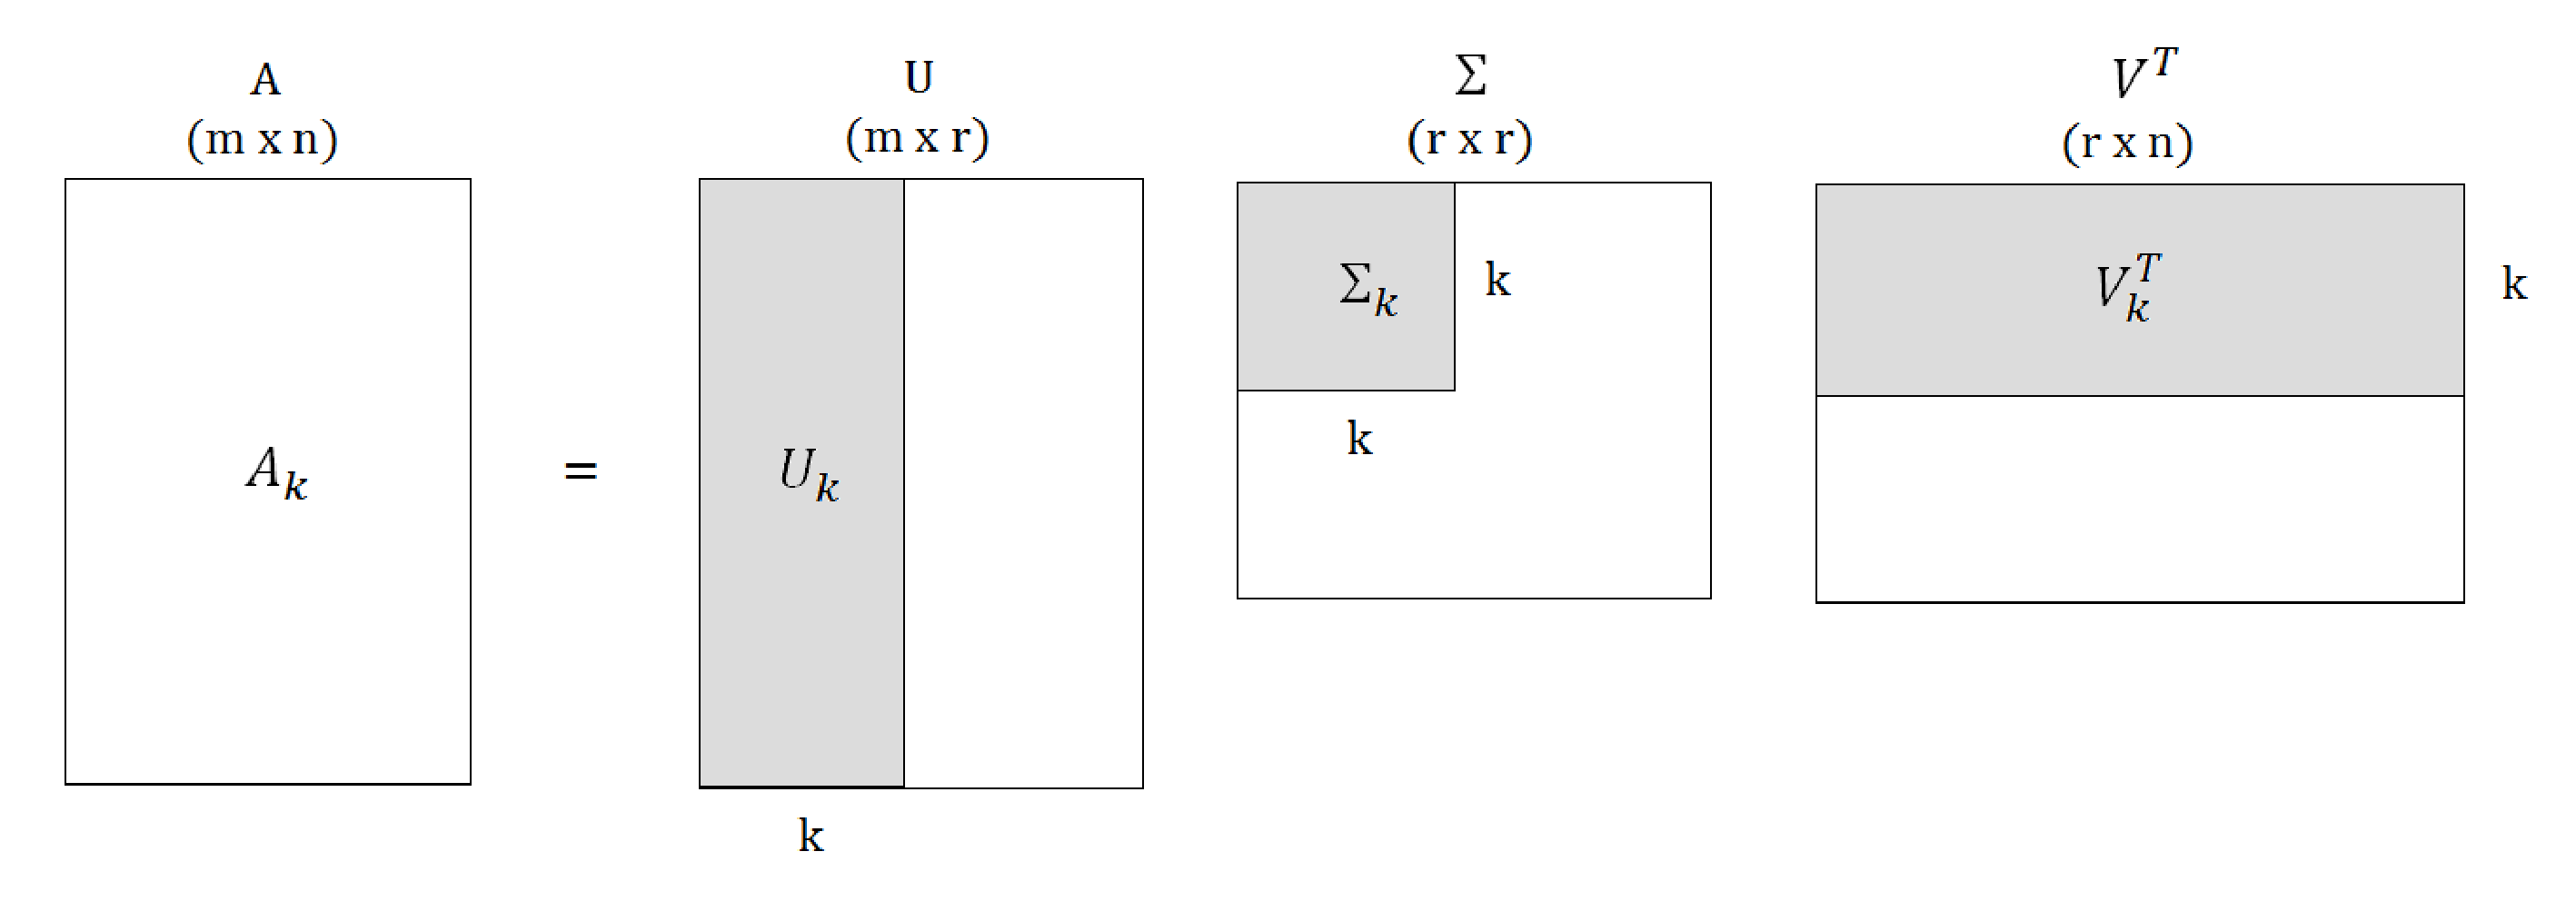
\includegraphics[width=\ScaleIfNeeded]{img/svd} 
 % or [scale=0.5]
	\caption[Diagram of truncated SVD]%
           {Diagram of truncated SVD}
\end{figure}
%
% description of the parameters in SVD diagram
%
\begin{tabular}{l l}
$A_{k}$ - best rank-$k$ approximation of $A$ & $m$ - number of terms\\
$U$ - term vectors & $n$ - number of documents \\
$\Sigma$ - singular values & $k$ - number of factors \\
$V^{T}$ - document vectors & $r$ - rank of $A$ \\
\end{tabular}
\end{center} 

Figure~\ref{lsa:truncated_svd} is a visual representation of \gls{SVD} as defined in equation~(\ref{lsa:svd}). $U$ and $V$ are considered as containing the term and document vectors respectively, and $\Sigma$ is constructed by the singular values of $A$. An imporant property of \gls{SVD} is that the singular values placed on the diagonal of $\Sigma$ are in decreasing order. Hence, if all but the first $k$ singular values are set to $0$, the semantic meaning in the resulting space is preserved to some approximation $k$, while noise or variability in word usage, is filtered out. Noise in this case are the terms with lowest weights which carry little meaning. By using fewer dimensions $k$, \gls{LSA} induces similarities amont terms including ones that have never occured together. Terms which occur in similar documents, for example, will be near each other in the k-dimensional space even if they never co-occur in the same document. This means that some documents which do not share any words with a users query may be near it in k-space.\\

A factor to be considered when computing \gls{SVD} is the run-time complexity of the algorithm. For decomposition of very large matrices, it is $O(n^2k^3)$, where $n$ is the number of terms in the text corpus, and $k$ is the number of dimensions in semantic space after dimensionality reduction. Note that $k$ is typically a small number between 50 and 350.\\

A more detailed description of \gls{SVD} can be found in \cite{Berry95usinglinear} and \cite{MatrixCompGolub96}.\\

\section{Querying the semantic space}
\label{lsa:querying_sspace}

In this work we are using \gls{LSA} for \gls{IR} purpose. Therefore, the final step of applying the technique is to pose queries on the constructed semantic space. A query $q$ is a set of words which must be represented as a document in the k-dimensional space, in order to be compared to other documents. The user's query can be represented by
%
% Query translation for LSA
%
\begin{equation}
\label{lsa:query}
q = q^{T}U_{k}\Sigma_{k}^{-1}
\end{equation}\\
where $q$ is the set of words in the query, multiplied by the reduced term and singular values matrices. Using the transformation in~(\ref{lsa:query}), the query is ''mapped'' onto the reduced k-space. After the mapping, the resulting query vector can be compared to the documents in the k-space, and the results ranked by their similarity or nearness to the query. A common similarity measure is the cosine between the query and the document vector. From the resulting document set, the documents closest to the query above certain treshold are returned. \\

\section{Factors influencing LSA performance}
\label{sec:lsa:factors_infl_lsa}
The effective usage of \gls{LSA} is a process of a sophisticated tuning. Several factors can influence the performance of the technique. These factors are pre-processing of texts~(removal of stop-words, filtering, stemming), frequency matrix transformations, choice of dimensionality $k$, choice of similarity measure.\\

Dumais et al.~\cite{dumais91improving} and Nakov et al.~\cite{Nakov_weightfunctions} have carried research on \gls{LSA} performance depending on the choice of factors such as frequency matrix transformations, similarity measures, and choice of dimension reduction parameter $k$. They conclude that performance based on the choice of these factors depends on the particular text corpus, as well as on the purpose of \gls{LSA} application. However, in the case of matrix transform, log-entropy performs better as compared to other matrix transform function combinations, including the popular term frequency - inverse document frequency~($tf\times idf$). Therefore, we implement the former in this work.
%
% entropy frequency matrix transformation
%
\begin{center}
\begin{tabular}{l l}
Local function:  & \multirow{2}{*}{ $ L(i,j)=\log(tf(i,j)+1) $ }\\
logarithm & \\
Global function: & \multirow{2}{*}{ $ G(i)=1+\frac{{\Sigma_{j}p(i,j)}}{\log n} $ } \\
entropy & \\
\end{tabular}
\end{center} 
where $n$ is the number of documents in the collection.\\

Further, it has been stated~(\cite{dumais91improving},\cite{NakovBetterResultsLSI}) that with respect to similarity measures used, \gls{LSA} performs optimal when cosine similarity measure is implemented to calculate the distance between vectors in the semantic space. We have therefore used it to measure the relevance between queries and documents. The cosine measure between two vectors $d_1$ and $d_2$ is given by:
%
% cosine similarity
%
\begin{equation}
\label{lsa:cosine_measure}
sim(d1,d2)=\frac{\overrightarrow{V}(d_1).\overrightarrow{V}(d_2)}{\left\vert \overrightarrow{V}(d_1) \right\vert.\left\vert \overrightarrow{V}(d_2)\right\vert}
\end{equation}

Dimensionality reduction parameter $k$ is defined empirically based on the experimentation results presented in Chapter~\ref{sec:implementation}. 
